% Use only LaTeX2e, calling the article.cls class and 12-point type.

\documentclass[12pt]{article}

\bibliographystyle{science}
% Users of the {thebibliography} environment or BibTeX should use the
% scicite.sty package, downloadable from *Science* at
% www.sciencemag.org/about/authors/prep/TeX_help/ .
% This package should properly format in-text
% reference calls and reference-list numbers.

\usepackage{scicite}

% Use times if you have the font installed; otherwise, comment out the
% following line.

\usepackage{times}

% The preamble here sets up a lot of new/revised commands and
% environments.  It's annoying, but please do *not* try to strip these
% out into a separate .sty file (which could lead to the loss of some
% information when we convert the file to other formats).  Instead, keep
% them in the preamble of your main LaTeX source file.


% The following parameters seem to provide a reasonable page setup.

\topmargin 0.0cm
\oddsidemargin 0.2cm
\textwidth 16cm 
\textheight 21cm
\footskip 1.0cm


%The next command sets up an environment for the abstract to your paper.

\newenvironment{sciabstract}{%
\begin{quote} \bf}
{\end{quote}}


% If your reference list includes text notes as well as references,
% include the following line; otherwise, comment it out.

\renewcommand\refname{References and Notes}

% The following lines set up an environment for the last note in the
% reference list, which commonly includes acknowledgments of funding,
% help, etc.  It's intended for users of BibTeX or the {thebibliography}
% environment.  Users who are hand-coding their references at the end
% using a list environment such as {enumerate} can simply add another
% item at the end, and it will be numbered automatically.

\newcounter{lastnote}
\newenvironment{scilastnote}{%
\setcounter{lastnote}{\value{enumiv}}%
\addtocounter{lastnote}{+1}%
\begin{list}%
{\arabic{lastnote}.}
{\setlength{\leftmargin}{.22in}}
{\setlength{\labelsep}{.5em}}}
{\end{list}}


% Include your paper's title here

\title{Death and taxa: time-invariant differences in mammal species duration}


% Place the author information here.  Please hand-code the contact
% information and notecalls; do *not* use \footnote commands.  Let the
% author contact information appear immediately below the author names
% as shown.  We would also prefer that you don't change the type-size
% settings shown here.

\author
{Peter D Smits,$^{1\ast}$\\
\\
\normalsize{$^{1}$Committee on Evolutionary Biology, University of Chicago,}\\
\normalsize{1025 E. 57th Stree, Culver Hall 402, Chicago, IL 60637, USA}\\
}

% Include the date command, but leave its argument blank.

\date{}



%%%%%%%%%%%%%%%%% END OF PREAMBLE %%%%%%%%%%%%%%%%



\begin{document} 

% Double-space the manuscript.

\baselineskip24pt

% Make the title.

\maketitle 



% Place your abstract within the special {sciabstract} environment.

\begin{sciabstract}
  Why species go extinct at different rates remains one of the most fundamental questions in paleobiology \cite{Simpson1944,VanValen1973,Raup1994,Quental2013,Wagner2014b}. Determining which and how biological traits influence extinction risk is vital for understanding the differential diversification of life during the Phanerozoic and for making predictions about species' vulnerability to anthropogenic impacts. Here I present a hierarchical Bayesian survival model of North American Cenozoic mammal species durations as predicted by species-level ecological factors, time of origination, and phylogenetic relationships. I also explicitly model the effect of species age on extinction risk, relaxing the Law of Constant Extinction which is the critical assumption underlying the Red Queen Hypothesis \cite{VanValen1973}. 
  This study focuses on time-invariant effects in an effort to characterize aspects of the selective patterns of background extinction in an effort to determine if the current biodiversity crisis is congruent with an intensification of previous processes or represents the arrival at an environmental ``tipping point'' \cite{Barnosky2011,Barnosky2012a} or a shift in ``macroevolutionary regime'' \cite{Jablonski1986} associated with a mass extinction.
\end{sciabstract}


% In setting up this template for *Science* papers, we've used both
% the \section* command and the \paragraph* command for topical
% divisions.  Which you use will of course depend on the type of paper
% you're writing.  Review Articles tend to have displayed headings, for
% which \section* is more appropriate; Research Articles, when they have
% formal topical divisions at all, tend to signal them with bold text
% that runs into the paragraph, for which \paragraph* is the right
% choice.  Either way, use the asterisk (*) modifier, as shown, to
% suppress numbering.

%\section*{Introduction}
Here I test how non-random extinction is with respect to organismal- and species-level traits during times of background extinction, if and which traits have time-invariant effects on species duration, and if extinction is taxon-age independent among Cenozoic mammals? These questions are dealth with using a single model of species duration and survival whose parameter estimates directly test these questions. 
Cenozoic mammals represent an ideal group and time period because their fossil record is well sampled, well resolved both temporally and spatially, and the ecology and taxonomy of individual species are generally understood \cite{Alroy2009,Liow2008,Smith2004,Quental2013,Simpson1944,Tomiya2013,Marcot2014}. 

Time-invariant factors are those, that when comparing taxa over a long period of time, there is a consistent effect that is generalizable over the entire period of interest. While the strength of the effect may vary over time, the direction does not change. These consistent effects reveal fundamental differences between selective regimes. Periods of background extinction represnt an opportunity to characterize the selective pattern of a given macroevolutionary regime given that they are relatively constant with changes occurring slowly \cite{Jablonski1986,Raup1988}.

The organismal- and species-level traits studied here are dietary and locomotor categories, bioprovince occupancy, and body mass. Each of these traits are related to different aspects of a species' adaptive zone such as homeostatic energetic cost, population density, expected home range size, set of potential prey items, and dispersal ability \cite{Smith2004,Jernvall2004}. It is expected that species with larger geographic ranges have lower extinction rates than species with smaller geographic ranges \cite{Jablonski1986,Roy2009c}. However, organismal traits directly related to species--environment interactions may play an important role in determining extinction risk. By modeling extinction via traits related to environmental preference, the relative importance of species- and organismal-level properties can be elucidated. These traits are analyzed in the context of both shared species origination cohort and phylogenetic position. From there the relative contribution of the three sources of variance (i.e. species, cohort, and phylogeny) to the total unexplained variance can be estimated. 

% this is were i could add a bit about methods

The parameter estimates of the model demonstrate that dietary category has a large amount of variation in the pairwise differences of effects on expected duration (Fig. \ref{subfig:diet}). Carnivory appears to be associated with a greater expected duration than herbivory or insectivory, while approximately equal to or less than the expected duration of an omnivore. Omnivory is associated with greater expected duration than either herbivory or insectivory. Finally, herbivory and insectivory are associated with approximately equal effects on expected duration. 
Given that carnivores and omnivores have approximately equal extinction risk, and it has been found previously that carnivores have a greater diversification rate than omnivores, this implies that carnivores have a greater origination rate than omnivores \cite{Price2012}. This comparison implies that herbivores, which have the greatest extinction risk, must also have a very high origination rate in order to have the greatest diversification rate of these three categories \cite{Price2012}. 

For locomotor category, arboreality appears to be associated with a lower expected duration than either scansoriality or a ground dwelling life habit (Fig. \ref{subfig:loco}). Scansoriality and a ground dwelling life habit have approximately equal expected durations. These results consistent with the hypotheses that arboreality is associated with a greater expected extinction risk than either with scansoriality and ground dwelling taxa. Importantly, scansoriality appears to not influence any difference in extinction risk when compared with ground dwelling taxa. This can be interpreted that arboreal taxa, which require a specific kind of environment, may be more prone to extinction because the lack of permanency of those environments preventing species persistence. 

The large difference in time-invariant extinction risk between omnivores and both herbivores and insectivores is most likely related to the concept of ``survival of the unspecialized'' where less specialized taxa have a lower expected extinction risk than specialized taxa \cite{Liow2004a,Simpson1944}. Because larger effects are easier to identify, the magnitude of this effect also explains both the early identification and origin of this hypothesis \cite{Simpson1944}. The lack of effect of body size on extinction risk is consistent with some previous results \cite{Tomiya2013}. The direction/sign of the modal estimate of effect is not consistent with the prediction of increase in extinction risk associated with increase in body size \cite{Liow2008}. However, the other studies were performed at the generic-level which may or may not involve different processes than at the species-level model \cite{Tomiya2013,Liow2008}.

As expected, bioprovince occupancy has the largest effect on expected species duration/extinction risk \ref{fig:eff_other}). Body size has near zero effect on expected duration, similar to the lack of relationship between body size and generic duration \cite{Tomiya2013}. 

Of the three sources of variance present in the model, individual species variance accounts for approximately 70\% of the observed variance (Fig. \ref{fig:vpc}). Both cohort and phylogenetic effects account for the other 30\% of the observed variance. While both of these effects are the source of approximately 15\% of observed variance individually, the total combined effect factors indicates that neither can be ignored. As \(VPC_{phylo}\), which is equivalent to phylogenetic heritability, is greater than 0 it is not appropriate to ignore phylogeny when modeling survival \cite{Housworth2004} as is commonly done in paleontological studies \cite{Alroy2009,Foote2013,Jablonski2006a,Hunt2007a,Liow2008,Payne2007}. 

The estimates for the individual cohort effects show a weak pattern of increased extinction risk in older Cenozoic cohorts and decreased extinction risk in younger cohorts (Fig. \ref{fig:eff_cohort}). However, this pattern is not very strong as there is a large amount of variation, particularity for older cohorts. For example, note the two cohorts between 50 and 55 My that have a much lower extinction risk than other cohorts of similar age. However, it is interesting to note that the apparent shift from older cohorts with a higher extinction risk to younger cohorts with lower extinction risk is approximately 30 Mya or the Paleogene--Neogene boundary. This transition is marked by the opening up of the landscape and the rise of grazers and the decline heavily forested environments. This shift may underly the inferred increased extinction risk associated with arboreal species compared to ground dwelling or scansorial species (Fig. \ref{subfig:loco}). However, because the model used here does not allow for change in time-invariant effects, I cannot identify this transition as a tipping point or shift in selective regime with any certainty \cite{Barnosky2012a,Barnosky2011}.

The estimate of the Weibull shape parameter, \(\alpha\), is greater than 1 meaning that extinction risk is expected to increase with taxon age (Table \ref{tab:post_sum}). The estimate of \(\alpha\) is also rather tightly constrained, having a small posterior standard deviation. \(\alpha\) is related to the strength of time on extinction risk and is a key parameter in the hazard function \(h(t)\) which can be interpreted as the rate, or approximate probability, of an individual of age \(t\) going extinct. As the value of \(\alpha\) is between 1 and 1.5, extinction risk for a given species only gradually increases with age. This result has two possible explanations: (1) older taxa being aged out or out competed by younger taxa, or (2) as an artifact of the minimum resolution of the fossil record.

The hypothesis that older taxa are being outcompeted or replaced by younger taxa is also consistent with the some recent results \cite{Wagner2014b,Quental2013}, both of which require that older taxa have a greater extinction risk than younger taxa. This is also consistent with the cohort effect (Fig. \ref{fig:eff_cohort}) where Paleogene cohorts may have been replaced or out-competed by younger, Neogene cohorts.

The other possible explanation for the inferred increase in extinction risk with species age is the minimum resolution which might cause an upward bias in estimates of the Weibull shape parameter \(\alpha\) \cite{Sepkoski1975}, an effect which can be observed by the initial plateau in the K-M estimate of \(S(t)\) for the observed (Fig. \ref{fig:ppc_surv}). This plateau is a hallmark of the original paleontological survival analyses \cite{VanValen1973} which was identified as partially a product of minimum resolution of the fossil records of the different studied groups.

Given this known biasing factor and previous results \cite{Wagner2014b,Quental2013}, I hypothesize that the inferred pattern is most likely a combination of these two explanations working on concert. In order to determine the relative importance of these two explanations, more work is required into approaches for directly modeling the minimum resolution of the fossil record.

One of the open questions in paleobiology and macroecology is whether the current biodiversity crisis qualified as a mass extinction \cite{Alroy2010,Barnosky2011,Barnosky2012a}. Because change in the magnitude of extinction risk is not necessarily the best indicator of a shift from background to mass extinction \cite{Wang2003}, it is more fruitful to look for changes in the direction of selection, loss of a selective pressure, or the appearance of novel selective pressures. Comparison of the estimated effects of organismal- and species-level traits analyzed here with previous studies demonstrates a mixture of congruence and incongruence. 

As expected, large range size is always associated with lower extinction risk in the Recent \cite{Fritz2009,Fritz2010b,Liow2009,Purvis2000a}. While I found that body size has no time-invariant effect on extinction risk, large body size is associated with increased extinction risk in the Recent, though this is variable across environments and clades \cite{Liow2009,Fritz2009,Purvis2000a}. A higher trophic level (e.g. carnivory versus herbivory) is associated with greater extinction risk in Primates and Carnivora \cite{Purvis2000a} which is not congruous with the results found here that carnivores have lower extinction risk than herbivores. Finally, phylogeny has been found to be a factor underlying current mammal species extinction risk, though this effect seems much greater in the Recent than for the whole Cenozoic \cite{Fritz2010b}. Note that the phylogeny of Recent mammals is much better than the primarily taxonomy based phylogeny used here, which may partially account for the difference in effect.

How many of these incongruities are within the standard range of time-variant effects is unknown, though these comparisons across multiple factors do point to our arrival at a tipping point \cite{Barnosky2012a,Barnosky2011} and potentially a shift in macroevolutionary regime \cite{Jablonski1986}.

There are a few data quality concerns in this study which are also inherent to almost any paleontological study. Almost all of the body mass estimates were obtained using published regression equations that estimate mass from some other body part (e.g. tooth). These estimates are known with error, which was not included in the model. If the standard deviation of the residuals from each of these regression equations was known, it would be possible to directly model this as measurement error \cite{Gelman2013d} though this greatly adds to model complexity and decreases some amount of interpretability. Incidentally, this has never been done in any paleontological studies. Also phylogeny used here is only a coarse, baseline estimate of the actual species relationships. Because of this, the analysis of phylogenetic effect on survival represents a minimum eistimate. As it stands though, these results point to the importance of including shared evolutionary history in diversification models.


There are many processes encompassed by background extinction and identifying the exact cause of any one species' reason for extinction is extremely difficult. By focusing on estimating the effects of different ecologies and historical factors on average extinction risk, it is possible to better understand what processes may have driven the resulting pattern of selection (i.e. diversity). Here, I focused on time-invariant factors and their relation to biological selectivity of extinction, possible reasons for the observed time-invariant effects, and the effects of taxon-age on extinction risk. I found that some organismal- and species-level traits such as omnivory and large geographic range size have time-invariant effects on mammal species extinction risk. I also found that there are small but non-ignorable effects of cohort and phylogeny. Finally, I found putative evidence of increasing extinction risk with species age, though this result may be partially due to the minimum resolution of the fossil record itself \cite{Sepkoski1975}.


\bibliography{newbib,packages}

% Following is a new environment, {scilastnote}, that's defined in the
% preamble and that allows authors to add a reference at the end of the
% list that's not signaled in the text; such references are used in
% *Science* for acknowledgments of funding, help, etc.

\begin{scilastnote}
\item Materials and methods are available as supplementary materials on Science Online. \label{supplement}
\item P.D.S would like to thank M. Foote, K. Angielczyk, R. Ree, P.D. Polly for discussion. J. Alroy and the Fossilworks/Paleobiology Database for data accumulation, entry, and availability. This is Fossilworks/Paleobiology Database publication number XXX.
\end{scilastnote}


% For your review copy (i.e., the file you initially send in for
% evaluation), you can use the {figure} environment and the
% \includegraphics command to stream your figures into the text, placing
% all figures at the end.  For the final, revised manuscript for
% acceptance and production, however, PostScript or other graphics
% should not be streamed into your compliled file.  Instead, set
% captions as simple paragraphs (with a \noindent tag), setting them
% off from the rest of the text with a \clearpage as shown  below, and
% submit figures as separate files according to the Art Department's
% instructions.

\clearpage

% latex table generated in R 3.1.2 by xtable 1.7-4 package
% Thu Jan  8 17:45:30 2015
\begin{table}[c]
  \centering
  \begin{tabular}{rrrrrrrrr}
    & mean & sd & 2.5\% & 25\% & 50\% & 75\% & 97.5\% & \(\hat{R}\) \\ 
    \hline
    alpha & 1.29 & 0.03 & 1.23 & 1.27 & 1.29 & 1.31 & 1.36 & 1.00 \\ 
    intercept & -0.78 & 0.14 & -1.05 & -0.87 & -0.78 & -0.68 & -0.51 & 1.00 \\ 
    logit(occupancy) & -0.53 & 0.08 & -0.69 & -0.59 & -0.53 & -0.48 & -0.38 & 1.00 \\ 
    log(size) & -0.05 & 0.05 & -0.14 & -0.08 & -0.05 & -0.01 & 0.05 & 1.00 \\ 
    ground dwelling & -0.28 & 0.10 & -0.47 & -0.34 & -0.28 & -0.21 & -0.09 & 1.00 \\ 
    scansorial & -0.22 & 0.11 & -0.43 & -0.29 & -0.22 & -0.14 & -0.00 & 1.00 \\ 
    herbivore & 0.09 & 0.09 & -0.09 & 0.03 & 0.09 & 0.14 & 0.27 & 1.00 \\ 
    insectivore & 0.10 & 0.11 & -0.11 & 0.03 & 0.10 & 0.17 & 0.31 & 1.00 \\ 
    omnivore & -0.12 & 0.11 & -0.33 & -0.19 & -0.12 & -0.05 & 0.09 & 1.00 \\ 
    \hline
    sd cohort & 0.33 & 0.06 & 0.23 & 0.29 & 0.33 & 0.37 & 0.48 & 1.00 \\ 
    sd phylogeny & 0.11 & 0.05 & 0.03 & 0.07 & 0.10 & 0.14 & 0.23 & 1.03 \\ 
    \hline
  \end{tabular}
  \caption{Marginal posterior estimates for the praameters of interested based on 1000 posterior samples. The intercept can be interpreted as the estimate for the mean observed species. The other values are the effect of a trait on the expected species duration as expressed as deviation from the mean. The categorical variables are binary index variables where an observation is of that category or not. \(\hat{R}\) values of less than 1.1 indicate approximate chain convergence for the posterior samples.}
  \label{tab:post_sum}
\end{table}



\begin{figure}[ht]
  %\centering
  %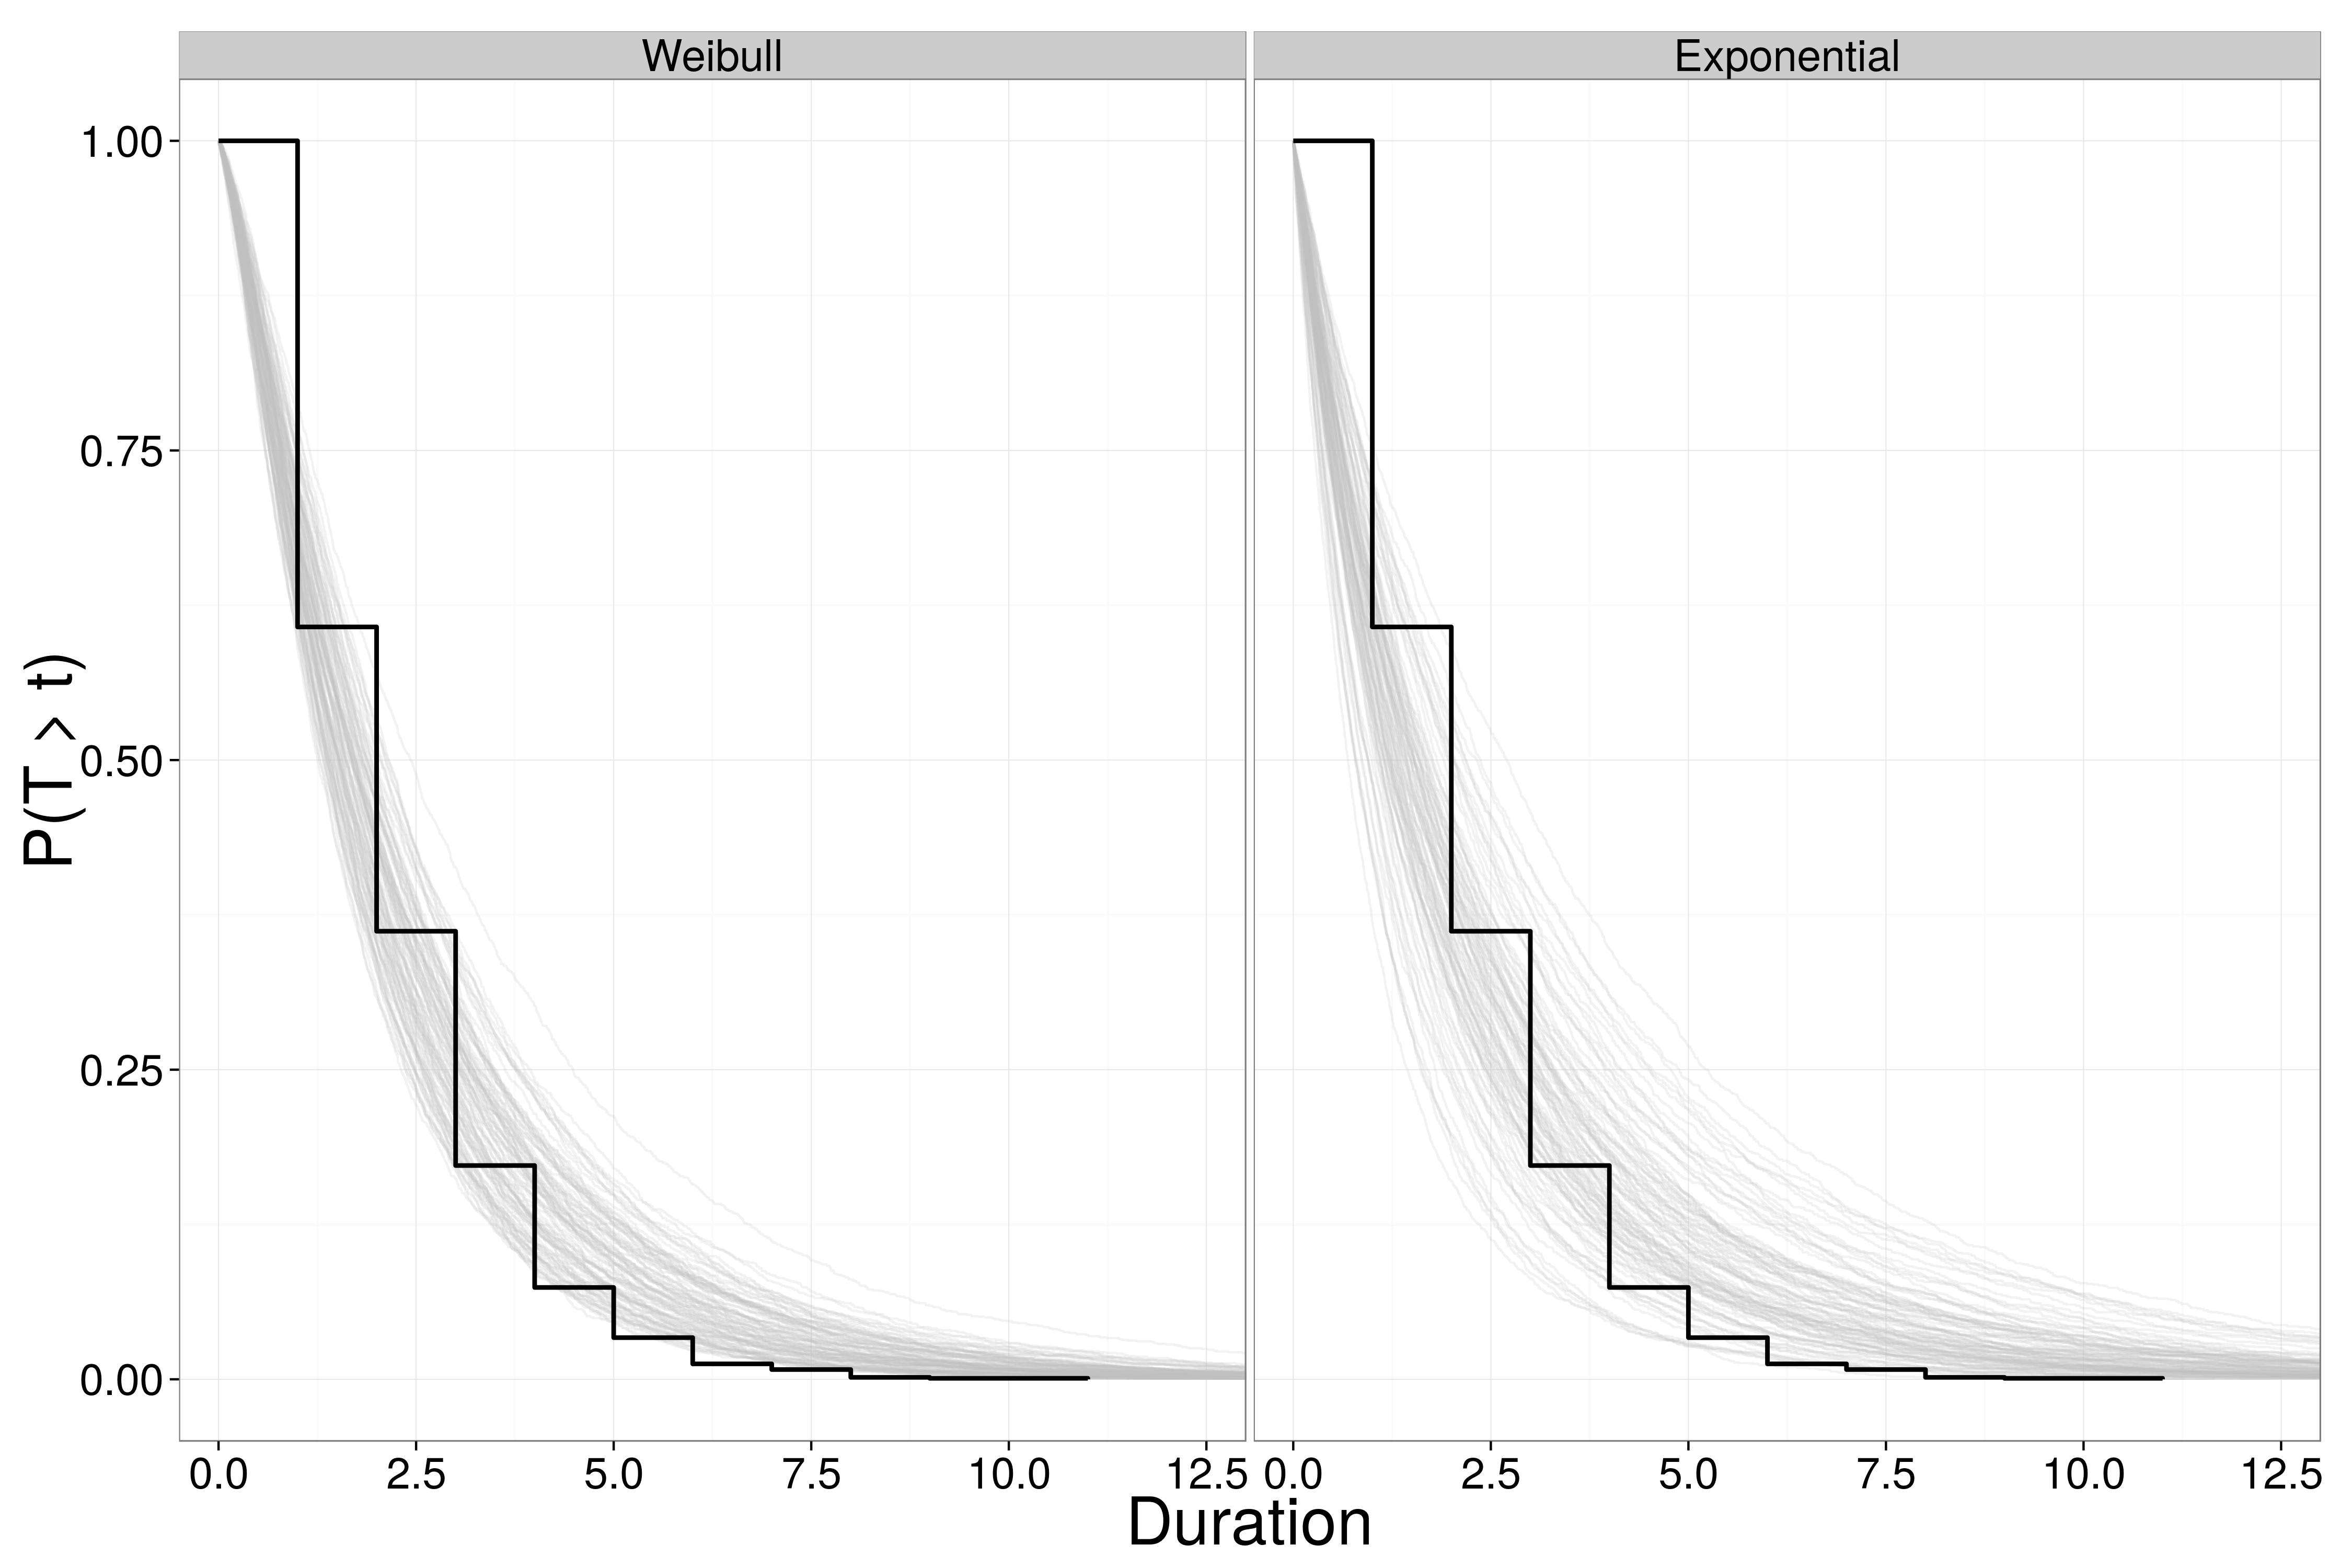
\includegraphics[height = 0.5\textheight, width = \textwidth, keepaspectratio = true]{figure/survival_function}
  \caption{Comparison between K-M estimate of survival function (black) from the observed versus K-M estimates from 100 simulated data sets using the fitted model (dark grey). Simulated data sets were generated by drawing parameter values randomly from their estimated posteriors and using the observed covariate information to estimate durations for all the observed species. On the left are the results from the full survival model, while on the right are the results from a simplified model where duration follows an exponential distribution and there is no phylogenetic effect.}
  \label{fig:ppc_surv}
\end{figure}


\begin{figure}[ht]
  %\centering
  %\begin{subfigure}[b]{0.4\textwidth}
  %  \caption{}
  %  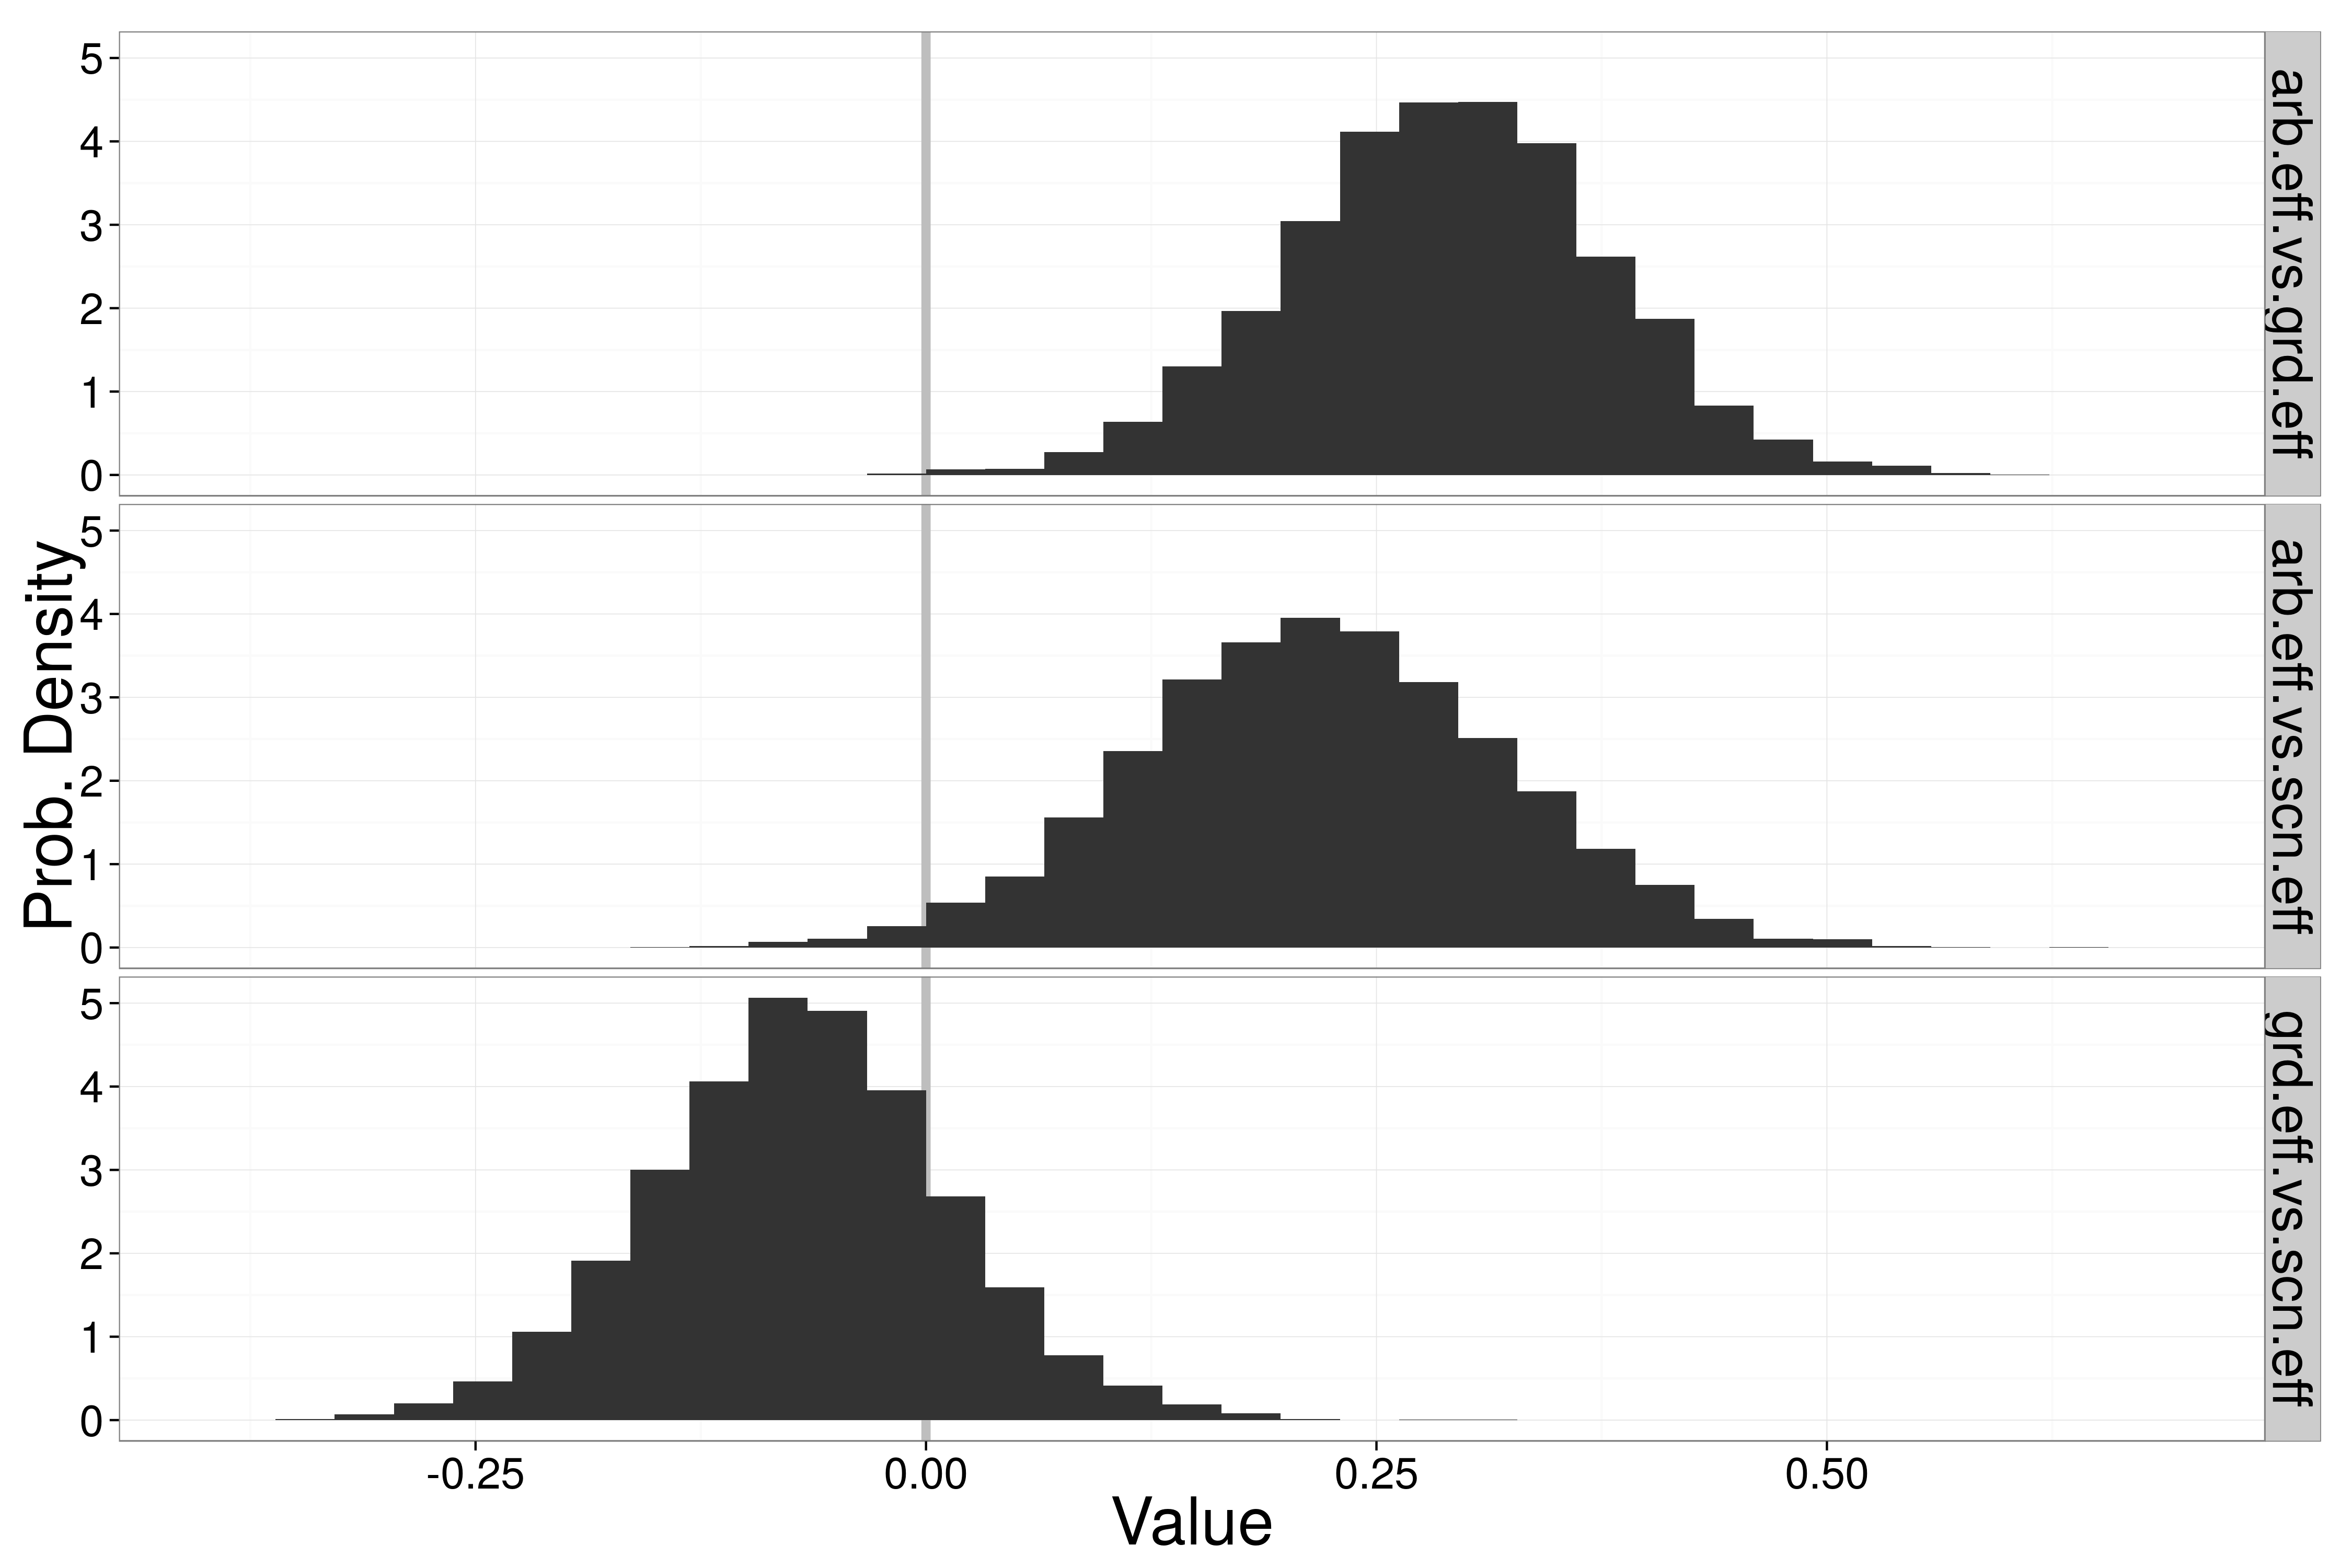
\includegraphics[height = 0.5\textheight, width = \textwidth, keepaspectratio = true]{figure/loco_diff_est}
  \label{subfig:loco}
  %\end{subfigure}
  %\begin{subfigure}[b]{0.4\textwidth}
  %  \caption{}
  %  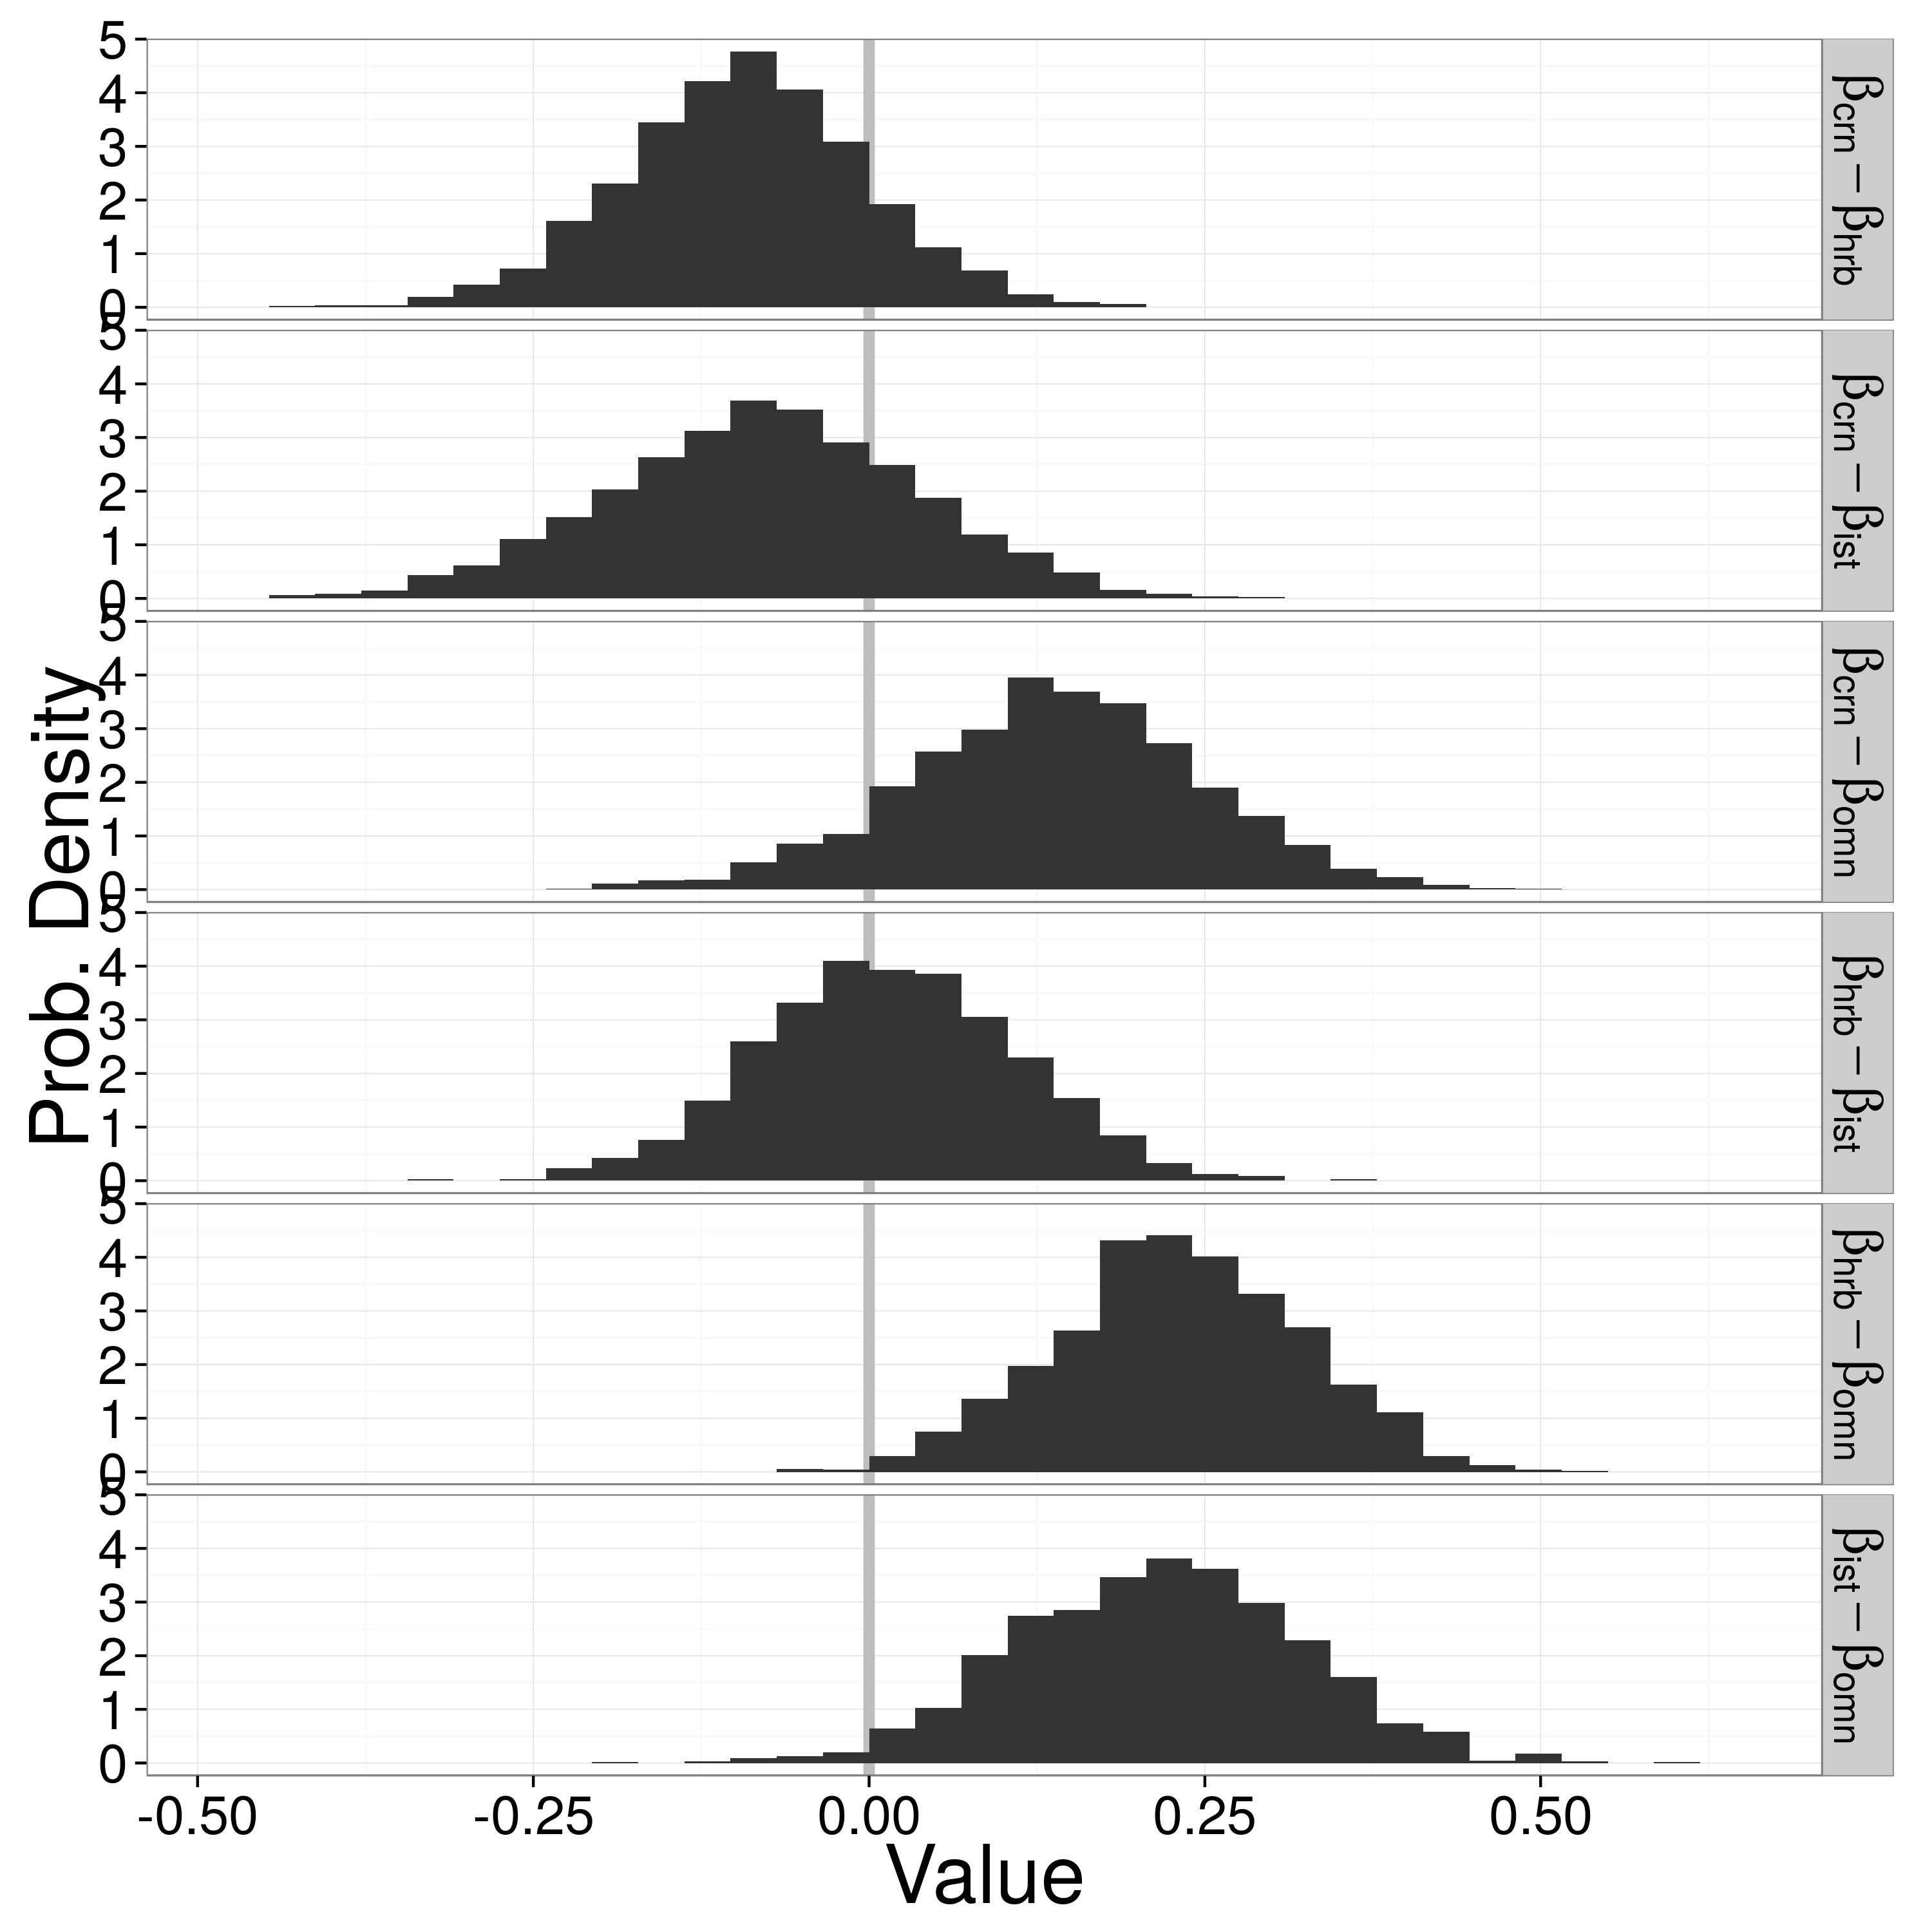
\includegraphics[height = 0.5\textheight, width = \textwidth, keepaspectratio = true]{figure/diet_diff_est}
  \label{subfig:diet}
  %\end{subfigure}
  \caption{Pairwise differences in effect of the locomotor (\ref{subfig:loco}) and dietary categories (\ref{subfig:diet}) on expected duration from 1000 samples from the posterior distribution. Comparisons of locomotor categories, from top to bottom (\ref{subfig:loco}), are: arboreal versus ground dwelling, arboreal versus scansorial, and ground dwelling versus scansorial. For dietary category, from top to bottom (\ref{subfig:diet}): carnivore versus herbivore, carnivore versus insectivore, carnivore versus omnivore, herbivore versus insectivore, herbivore versus omnivore, and insectivore versus omnivore. Values to the left indicate that the first category is expected to have a greater duration than the second, while values to the right indicate that the first category is expected to have a shorter duration.}
  \label{fig:trait_est}
\end{figure}

\begin{figure}[ht]
  %\centering
  %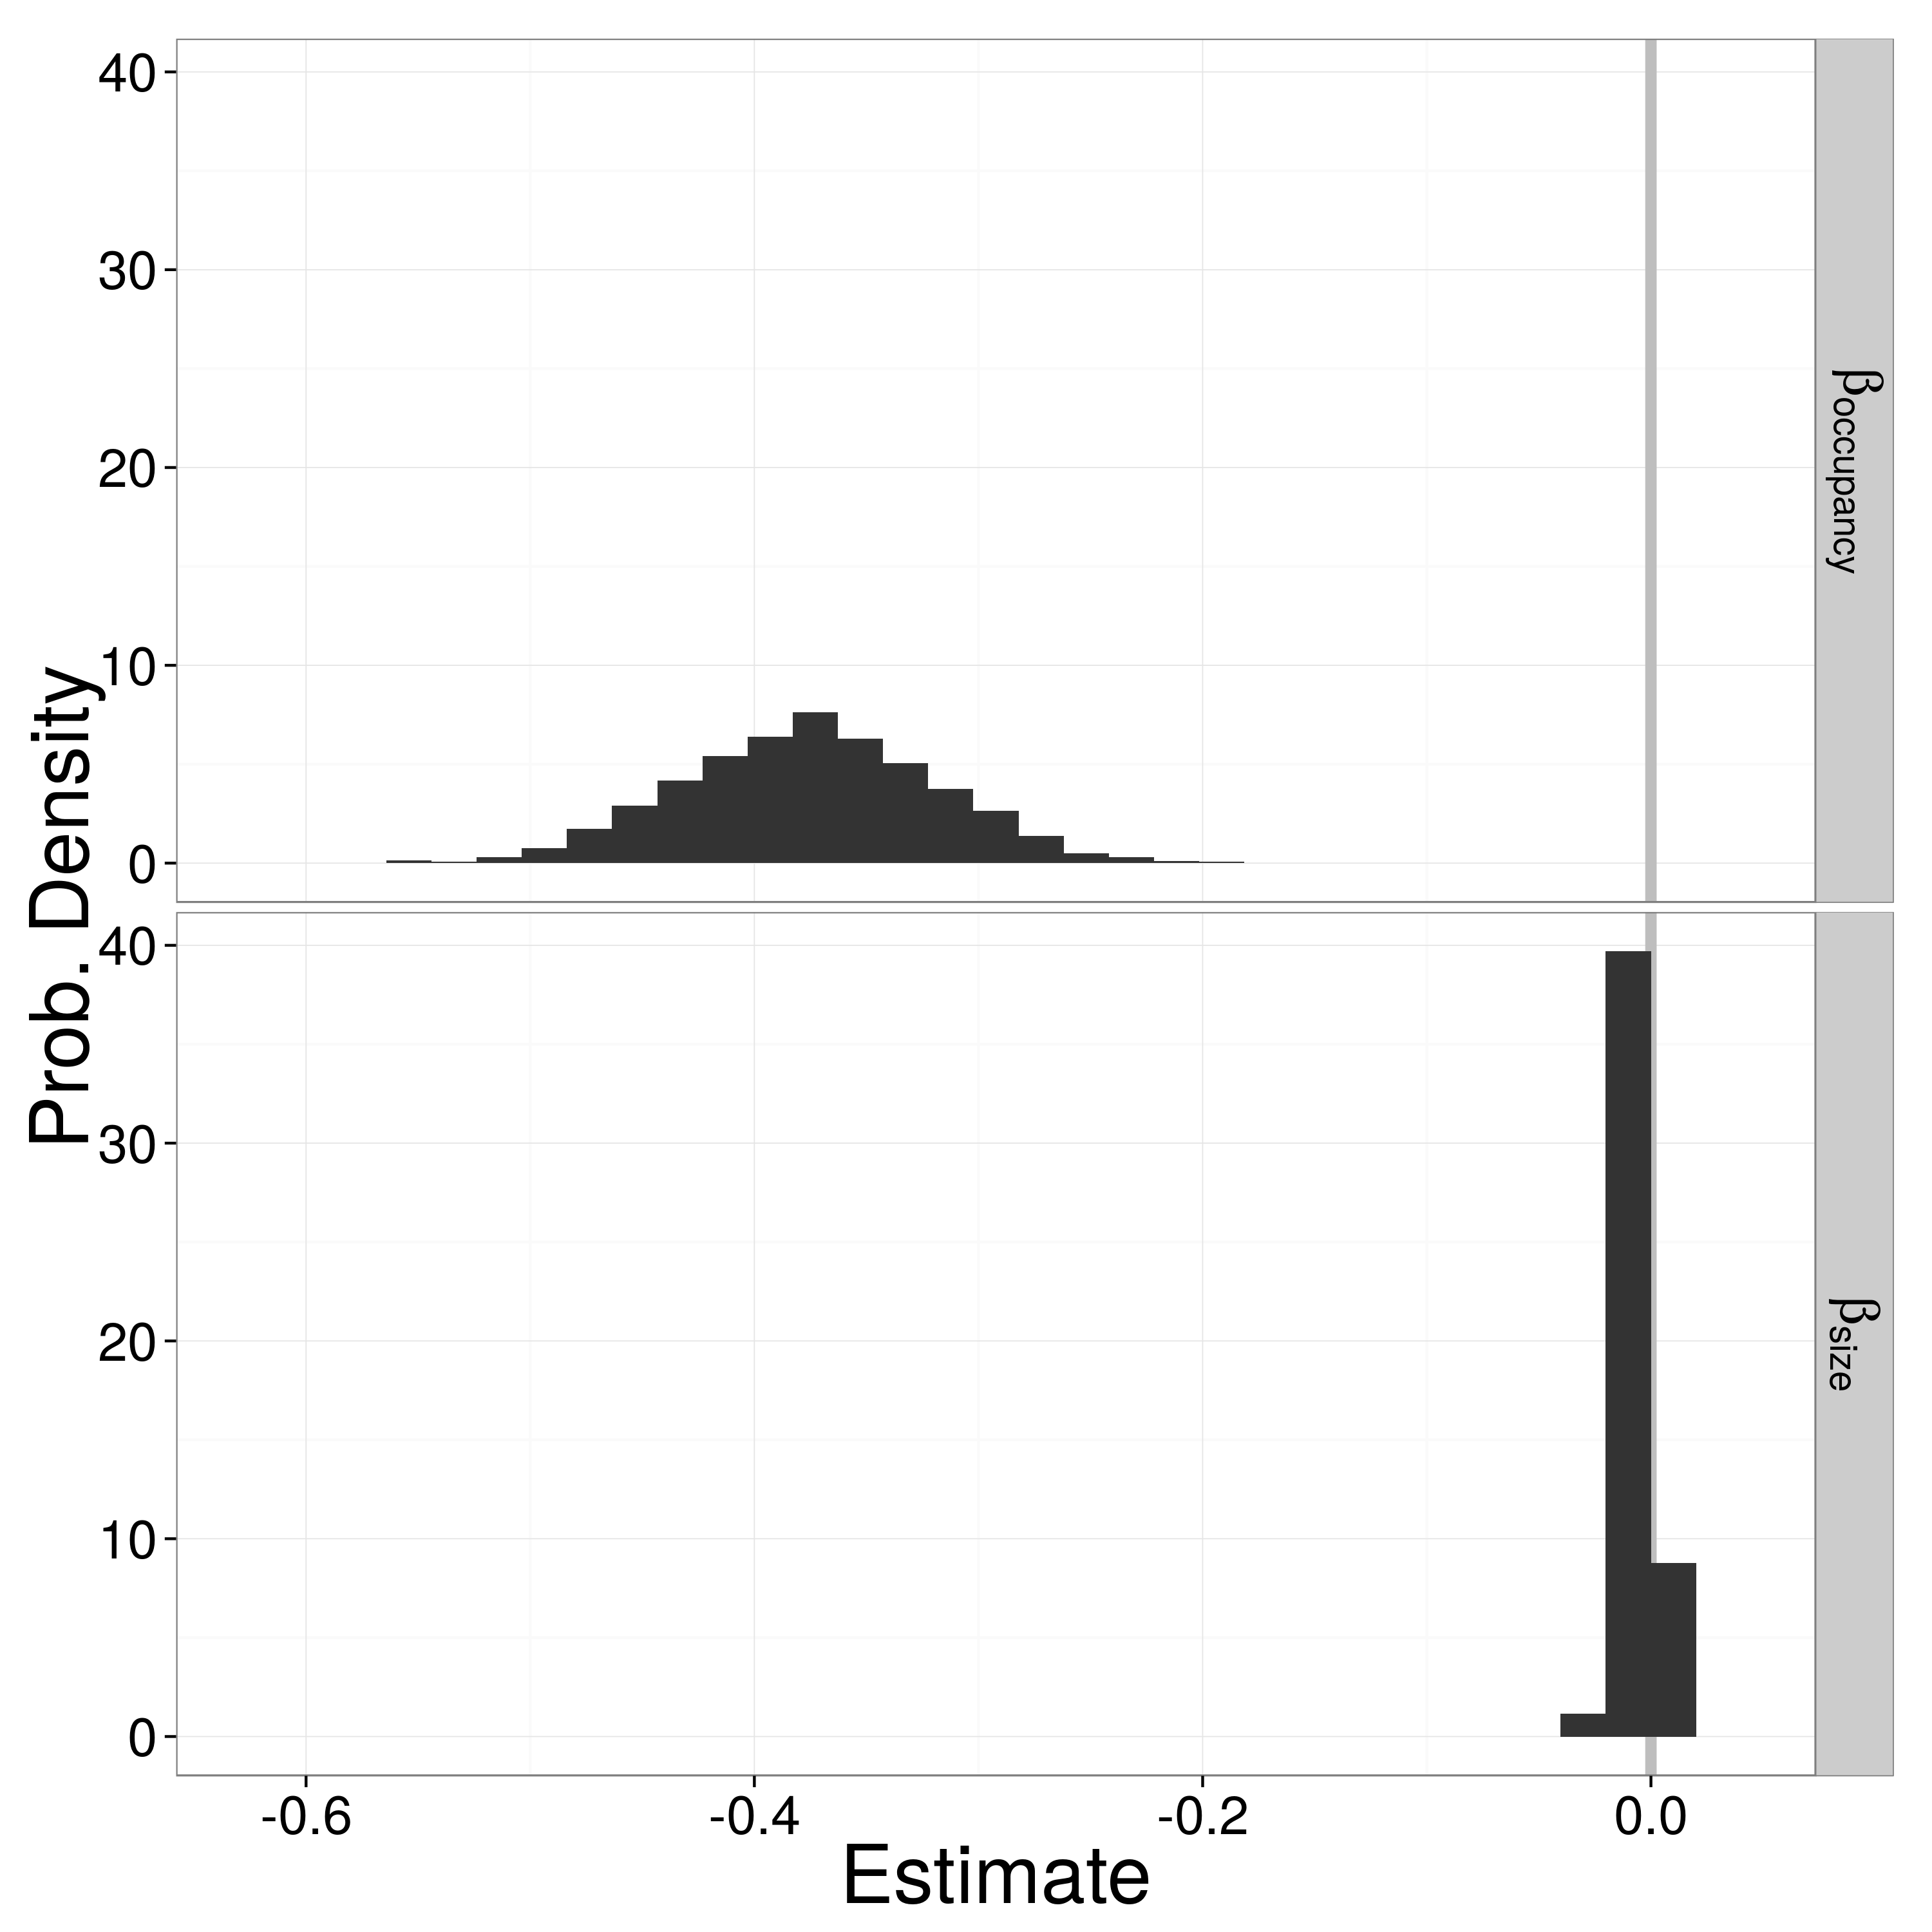
\includegraphics[height = 0.5\textheight, width = \textwidth, keepaspectratio = true]{figure/other_est}
  \caption{}
  \label{fig:eff_other}
\end{figure}

\begin{figure}[ht]
  %\centering
  %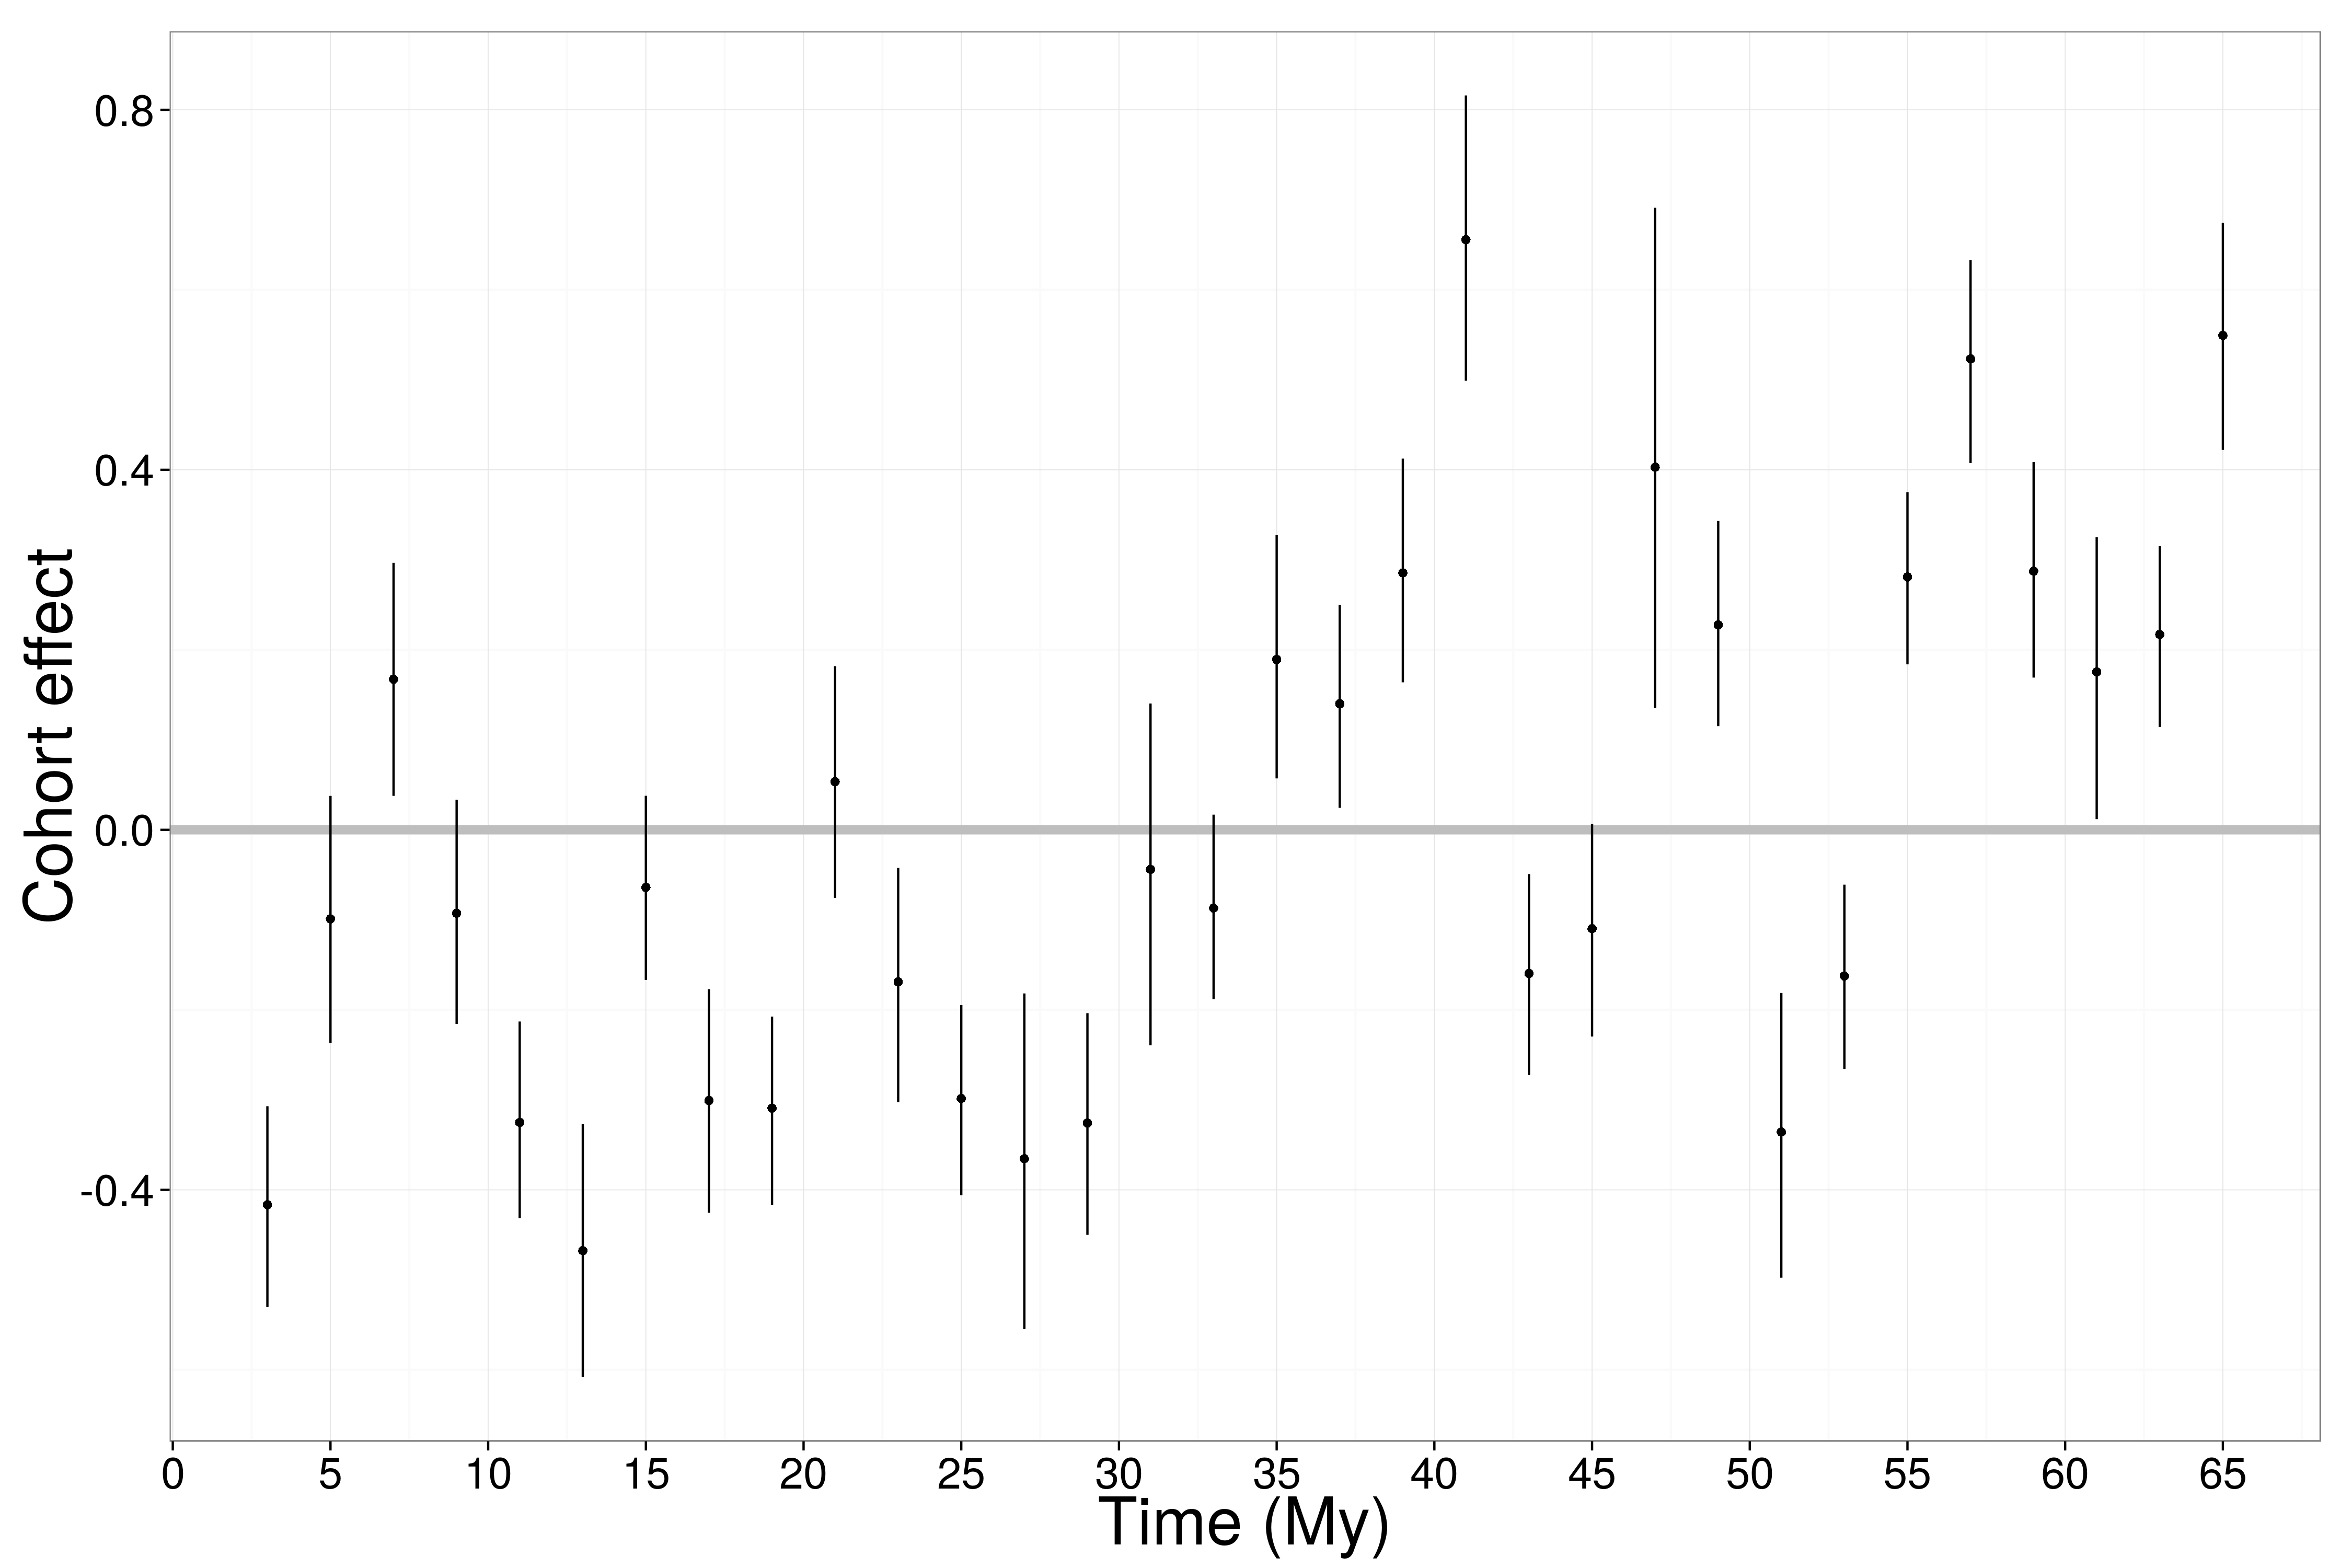
\includegraphics[height = 0.5\textheight, width = \textwidth, keepaspectratio = true]{figure/cohort_est}
  \caption{Summaries of posterior estimates of individual cohort effect depicted as medians and 80\% credible intervals. High values correspond to shorter species durations while lower values correspond to greater species durations compared to the mean duration. Lines are placed at the middle of the 2 My origination cohorts.}
  \label{fig:eff_cohort}
\end{figure}

\begin{figure}[ht]
  %\centering
  %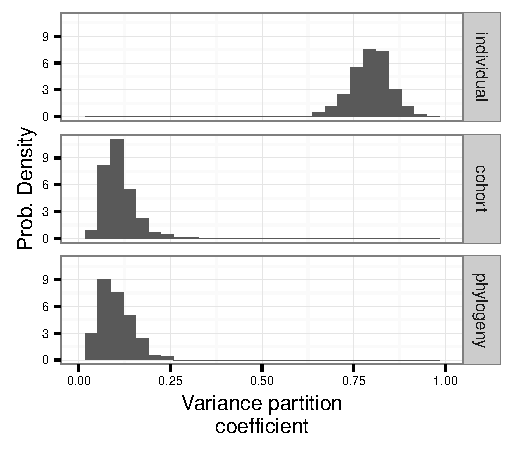
\includegraphics[height = 0.5\textheight, width = \textwidth, keepaspectratio = true]{figure/variance_est}
  \caption{Estimates of the variance partitioning coefficients for the three different sources of variance: species, cohort, and phylogeny. Higher values correspond to greater contribution to total observed variance. Each of the estimates is a distribution of 1000 approximating simulations due to the model's non-normally distributed errors.}
  \label{fig:vpc}
\end{figure}

\end{document}
